\section{Fold geometry, automatic regularity, and semi-global realization}
\label{sec:analytic-global-structure}

The auxiliary potential does more than shorten the velocity-field equation.
It identifies the exact discriminant at which the physical inverse problem
changes sheet, imports global tools from harmonic analysis, and makes the
logical gap between analytic local construction and smooth classical
solutions disappear. Throughout this section, $D$ denotes a connected
domain contained in $\{r>0,\eta>0\}$ and
$$
A=\partial_\eta\Phi_{\ellzero}(r,\eta)
=2+\ellzero r\left(\frac1v-v\right).
$$

\subsection{The density boundary as a Whitney fold}

Let $x=r\ellzero$ and let $\mathcal N_v(x)$ be the algebraic density
polynomial in Eq.~\eqref{eq:density-polynomial}. Direct factorization gives
\begin{equation}
\mathcal N_v(x)
=vA\bigl[2v-(1+v^2)x\bigr].
\label{eq:density-fold-factorization}
\end{equation}
The two factors in Eq.~\eqref{eq:density-fold-factorization} have different
geometric meanings: the second is an ordinary zero of the density factor,
whereas the first is the Jacobian of the point linearisation.

\begin{theorem}[Density fold and physical inverse sheet]
\label{thm:density-whitney-fold}
Fix $0<v_0<1$ and a point $(r_0,\eta_0)$ with $\eta_0=r_0v_0$. At the lower
density root
$$
r_0\ellzero=-\frac{2v_0}{1-v_0^2},
$$
the map
$$
(r,\eta)\longmapsto\bigl(r,\Phi_{\ellzero}(r,\eta)\bigr)
$$
has a nondegenerate Whitney fold. Strictly positive density implies $A>0$
and therefore selects the orientation-preserving inverse sheet. A generic
transverse auxiliary datum has a square-root inverse at the fold; a smooth
crossing requires the pulled-back discriminant to admit a smooth square root
compatible with one continuous choice of sheet.
\end{theorem}

\begin{proof}
Equation~\eqref{eq:density-fold-factorization} shows that the lower root is
exactly $A=0$. At that root $\ellzero<0$, and
$$
\partial_{\eta\eta}\Phi_{\ellzero}
=-\ellzero\left(1+\frac1{v_0^2}\right)>0.
$$
Thus the derivative in the kernel direction vanishes simply while the
second derivative in that direction does not. The first component of the
map is $r$ itself, so the parameter-dependent Morse lemma gives local
coordinates $(R,S)$ in source and $(R,Y)$ in target for which the map is
$(R,S)\mapsto(R,S^2)$. This is the Whitney-fold normal form. Between the
two simple density roots, both factors on the right-hand side of
Eq.~\eqref{eq:density-fold-factorization} are positive, hence $A>0$.
Finally, inversion of $Y=S^2$ is generically $S=\pm\sqrt{Y}$. A smooth
inverse exists only when the pulled-back discriminant is a square in the
local smooth ring, with a coherent choice of sign. Along a one-dimensional
transverse slice, finite even vanishing order with positive leading
coefficient is sufficient for such a smooth signed square root. In the
analytic category the corresponding condition is local analytic
factorisation as a square; contact parity alone is not asserted to be
sufficient in several variables.
\end{proof}

\begin{remark}
The theorem is local. It does not say that every even-contact datum produces
a globally admissible metric, and it does not identify the fold with an
optical caustic. In particular, metric regularity must be checked after the
inverse is reconstructed; it cannot be inferred from the square-root model
alone.
\end{remark}

\begin{figure*}[t]
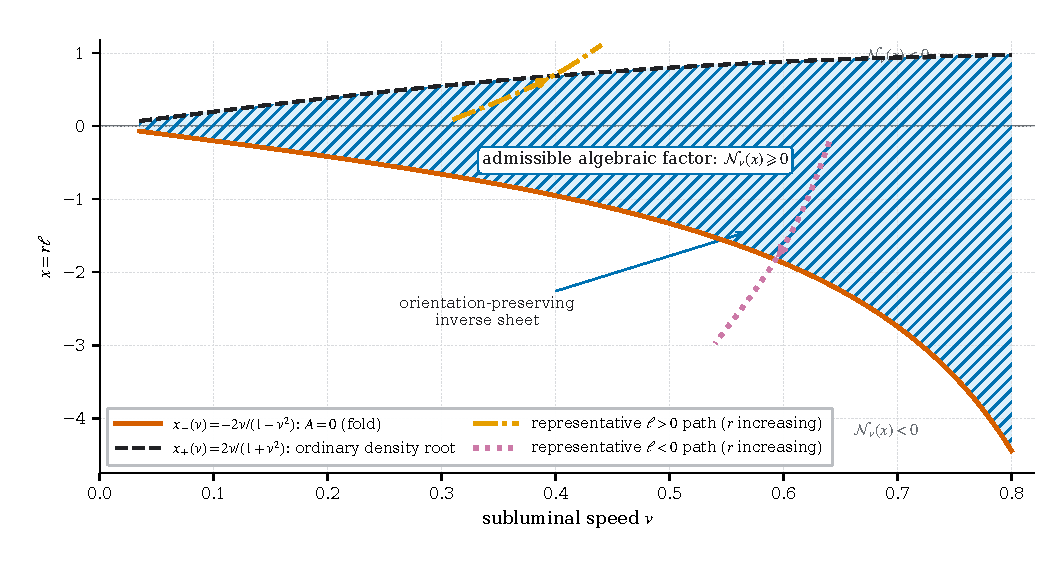
\includegraphics[width=\textwidth]{figures/density_admissibility_phase.pdf}
\caption{Exact density-admissibility diagram in the variables
$0<v\leqslant0.8$ and $x=r\ell$. At a regular noncritical point, the
hatched strip $x_-(v)\leqslant x\leqslant x_+(v)$ is equivalent to
$\rho\geqslant0$. The lower boundary is simultaneously $A=0$, the
Whitney fold of the point-linearising map, whereas the upper boundary is
an ordinary zero of the algebraic density factor. The dash-dotted and
dotted curves illustrate only the kinematics of $x=r\ell$ for fixed-sign
$\ell$ as $r$ increases; they are not solutions of the VFE. Thus the
diagram selects a local inverse sheet but does not establish a global
spacetime.}
\label{fig:density-admissibility-phase}
\end{figure*}

\subsection{Automatic analyticity and plateau propagation}

\begin{theorem}[Automatic analyticity and connected-sheet rigidity]
\label{thm:automatic-analyticity}
Let $\eta\in C^2(D)$ solve the exact constant-$\ell$ VFE and suppose
$A\neq0$ on $D$. Then $\eta$, $v$, and the locally reconstructed metric are
real analytic. If $\eta$ is constant on a nonempty open subset of $D$, then
it is constant throughout $D$.
\end{theorem}

\begin{proof}
Set $\mathcal F=\Phi_{\ellzero}(r,\eta)$. The exact chain-rule identity
behind Eq.~\eqref{eq:GS-operator} gives $\mathcal L\mathcal F=0$ in the
classical, hence distributional, sense. The operator $\mathcal L$ is
uniformly elliptic on every relatively compact subdomain of $D$ and has
analytic coefficients. Analytic elliptic regularity therefore makes
$\mathcal F$ real analytic~\cite{MorreyNirenberg1957CPAM}. Since $A$ never
vanishes, the analytic implicit-function theorem makes $\eta$ and $v$
analytic. The algebraic Killing block and the closed reconstruction
quadrature are then analytic as well.

Suppose $\eta=\eta_0$ on a nonempty open set. The comparison function
$$
\mathcal F_0(r)=\Phi_{\ellzero}(r,\eta_0)=c_0+c_2r^2
$$
is $\mathcal L$-harmonic. Unique continuation applied to
$\mathcal F-\mathcal F_0$ gives $\mathcal F=\mathcal F_0$ on $D$. Local
inverse uniqueness makes the set $\{\eta=\eta_0\}$ both open and closed in
$D$, and connectedness completes the proof.
\end{proof}

Strict positive density forces $A>0$ by
Eq.~\eqref{eq:density-fold-factorization}. Thus no analyticity assumption is
needed anywhere inside a strictly positive-density regular sheet. Plateau
propagation can stop only at a genuine boundary, the axis, $\eta=0$, the
fold, a change of equations, or loss of classical regularity.

\subsection{Exact elliptic Cauchy instability}

The preceding theorem is a regularity statement, not a stability theorem.
The following sequence quantifies the distinction for the precise operator
used here.

\begin{theorem}[Bessel--Hadamard instability]
\label{thm:bessel-hadamard}
For $k>0$, define
$$
\mathcal F_k(r,z)=e^{-\sqrt{k}}rJ_1(kr)\cosh(kz).
$$
Then $\mathcal L\mathcal F_k=0$. On every compact annulus
$I=[r_1,r_2]\Subset(0,\infty)$, the Cauchy data at $z=0$ converge to zero
in every fixed $C^m$ and Sobolev norm, while at every fixed $z_0>0$ their
$L^2(I)$ norm diverges. Consequently, continuation from smooth Cauchy data
to any collar of positive depth is discontinuous.
\end{theorem}

\begin{proof}
The Bessel equation for $J_1$ gives
$$
\left(\partial_r^2-\frac1r\partial_r\right)
\bigl[rJ_1(kr)\bigr]=-k^2rJ_1(kr),
$$
which cancels $\partial_z^2\cosh(kz)=k^2\cosh(kz)$. At $z=0$ the normal
datum vanishes, while every fixed radial derivative of the Dirichlet datum
is bounded by a polynomial in $k$ times $e^{-\sqrt{k}}$ on $I$; hence all
fixed smooth and Sobolev norms tend to zero. Standard large-argument Bessel
asymptotics~\cite{NISTDLMF} give an $L^2(I)$ norm bounded below by a fixed
negative power of $k$ along all sufficiently large $k$. Multiplication by
$e^{-\sqrt{k}}\cosh(kz_0)$ therefore makes that norm diverge exponentially.
If a continuous Cauchy solution map to the collar existed, this null
sequence of data would have a bounded image, a contradiction.
\end{proof}

Analytic data with Fourier decay $Me^{-a|\xi|}$ can be continued only to
depth $d<a$ with a conditional model rate
$O(M^{d/a}\varepsilon^{1-d/a})$. This observation describes the mechanism;
regularisation and numerical conditioning are reserved for Part II.

\subsection{Five-dimensional lift and a global rigidity theorem}

\begin{proposition}[$SO(5)$ harmonic lift]
\label{prop:five-dimensional-lift}
Writing $\mathcal F=r^2U$ gives
\begin{equation}
\mathcal L\mathcal F
=r^2\left(U_{rr}+\frac3rU_r+U_{zz}\right).
\label{eq:five-dimensional-lift}
\end{equation}
Thus $U(|y|,z)$ is harmonic on $\mathbb R^4_y\times\mathbb R_z$ wherever
$\mathcal F$ is $\mathcal L$-harmonic. With
$R=(r^2+z^2)^{1/2}$, Kelvin inversion is
$$
\mathcal F^K(r,z)
=R\mathcal F\left(\frac r{R^2},\frac z{R^2}\right).
$$
The regular and decaying $SO(4)$-invariant multipoles are
$$
\mathcal F_n^{\rm reg}=r^2R^nC_n^{3/2}(z/R),
\qquad
\mathcal F_n^{\rm dec}=r^2R^{-n-3}C_n^{3/2}(z/R).
$$
\end{proposition}

\begin{proof}
Equation~\eqref{eq:five-dimensional-lift} follows by differentiating
$r^2U$. The remaining statements are the five-dimensional Kelvin transform
and the zonal harmonic expansion, multiplied by $r^2$.
\end{proof}

\begin{theorem}[Global regular-axis rigidity for $\ellzero=0$]
\label{thm:ellzero-liouville}
Suppose the $\ellzero=0$ branch occupies the complete orbit half-plane, has
a regular axis and no finite boundary, puncture, additional end, horizon,
or singular axis segment. Assume, locally uniformly in $z$,
$|\eta(r,z)|\leqslant C_Kr^2$ near the axis and, for sufficiently large
$R=(r^2+z^2)^{1/2}$,
$$
|\eta(r,z)|\leqslant A\frac rR.
$$
Then $\eta\equiv0$. After stationary and meridional normalisation, the
spacetime is Minkowski and the dust density vanishes.
\end{theorem}

\begin{proof}
For $\ellzero=0$, set $U=2\eta/r^2$. The local axis estimate makes $U$
bounded near the lifted axis. That axis has removable capacity for bounded
harmonic functions in five dimensions, so $U$ extends harmonically across
it. On a lifted sphere of radius $S$, the asymptotic estimate and the
$\sin^3\theta$ angular measure give an $O(S^{-2})$ spherical $L^1$ mean.
The Poisson formula bounds $|U(X)|$ at each fixed interior point by
$O(S^{-2})$. Letting $S\to\infty$ gives $U(X)=0$. Hence $\eta=0$; the
remaining algebraic relations and quadratures give the stated normalised
metric and density.
\end{proof}

The domain hypotheses are essential. The theorem does not exclude a bounded
dust body stopped at a finite surface and matched to vacuum.

\subsection{Runge realization and formal integrability}

\begin{theorem}[Semi-global realization on a protected physical core]
\label{thm:runge-realization}
Let $K\Subset K'\Subset D_0\Subset D_1\Subset\{r>0\}$, and let
$\mathcal F_0$ be $\mathcal L$-harmonic near $K'$. Assume the elliptic
Runge no-compact-hole condition for the pair $(K',D_1)$. Then, for every
integer $m\geqslant0$ there are
$\mathcal L$-harmonic functions $\mathcal F_j$ on $D_1$ converging to
$\mathcal F_0$ in $C^m(K)$. If the inverse sheet on $K$ has quantitative
margins
$$
A\geqslant a_0>0,\qquad 0<v\leqslant1-\delta,
\qquad \rho\geqslant\rho_0>0,
$$
then, for $m\geqslant2$ and a fixed local normalization of the $\mu$
quadrature on each connected core, sufficiently accurate approximants
invert on the same sheet and retain these inequalities, with smaller
positive margins, on $K$.
\end{theorem}

\begin{proof}
The first assertion is the Lax--Malgrange Runge theorem for elliptic
operators with unique continuation~\cite{Malgrange1956AIF}, applied on the
larger compact set $K'$. Elliptic interior estimates then promote uniform
approximation near $K'$ to $C^m(K)$. For $m\geqslant2$, the implicit
inverse, its required first derivatives, the normalized local quadrature,
and the density depend continuously on the relevant finite jet on $K$ as
long as $A\geqslant a_0$. Openness of the three strict inequalities proves
the second assertion.
\end{proof}

No physical conclusion is asserted on $D_1\setminus K$. In particular,
Runge approximation neither preserves an exactly flat trace nor supplies an
asymptotically flat exterior or a matching surface.

\begin{theorem}[Regular-sheet involutivity and fold rank jump]
\label{thm:regular-sheet-involutivity}
Regard the exact VFE as a hypersurface in $J^2(D,\mathbb R_v)$. On
$A\neq0$, its order-two symbol is
$$
\sigma_2(\xi)=A(\xi_r^2+\xi_z^2),
$$
its Cartan characters are $(2,0)$, and the prolonged point transformation
$\mathcal F=\Phi_{\ellzero}(r,rv)$ identifies it with the prolonged linear
equation $\mathcal L\mathcal F=0$. At $A=0$, the symbol rank falls from one
to zero and $\dim g_2$ jumps from two to three. Appending
$v_r=v_z=0$ makes every positive constant-field branch inconsistent; the
first prolongation leaves only $\ellzero=v=0$.
\end{theorem}

\begin{proof}
The principal part of the VFE is $A(v_{rr}+v_{zz})$. Its kernel in
$S^2T^*D$ is the two-dimensional space of trace-free quadratic forms. Its
successive prolongations are the homogeneous harmonic polynomials in two
variables and remain two-dimensional, giving characters $(2,0)$. On
$A\neq0$ the point map is a jet diffeomorphism, so formal integrability and
involutivity follow constructively from the linear equation. When $A=0$ no
second derivative remains in the symbol, so $g_2=S^2T^*D$ has dimension
three. Finally, $v_r=v_z=0$ kills their first prolongations, while the VFE
reduces to $\ellzero r-v=0$; differentiation in $r$ gives $\ellzero=0$ and
then $v=0$.
\end{proof}

This last calculation is also recorded as a branch-sensitive
`rifsimp()`/Thomas certificate. Its differential-algebra output is evidence
for the encoded local system; it does not establish positivity, global
existence, or boundary regularity.
